\section{Background}

\subsection{Background of Remote Sensing}

Since the development of remote sensing technology in the early 20th century, it has undergone significant technological advancements and application expansions. The earliest applications of remote sensing technology can be traced back to photogrammetry techniques using balloons and airplanes\cite{bastiaanssenRemoteSensingIrrigated2000}. After World War II, with the advancement of space technology, satellite remote sensing gradually became mainstream. In 1972, the United States launched the first Earth Resources Technology Satellite (Landsat-1), marking the beginning of the modern satellite remote sensing era. Subsequently, various countries launched multiple remote sensing satellites, such as France's SPOT series\cite{SPOTsate81:online}, Japan's ALOS series\cite{Advanced84:online}, and Europe's Sentinel series\cite{Sentinel88:online}. These satellites have greatly enhanced the capability to acquire and apply remote sensing data.

\begin{figure}[htbp!]
    \centering
    \begin{subfigure}[b]{0.15\textwidth}
        \centering
        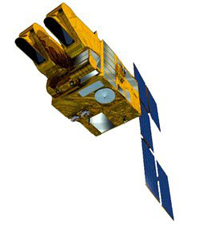
\includegraphics[height=0.1\textheight]{figs/Spot-5.jpg}
        \caption{SPOT}
    \end{subfigure}
    \begin{subfigure}[b]{0.15\textwidth}
        \centering
        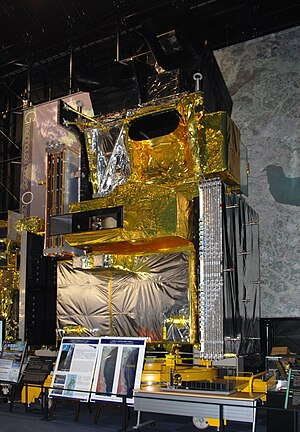
\includegraphics[height=0.1\textheight]{figs/AlOS.jpg}
        \caption{ALOS}
    \end{subfigure}
    \begin{subfigure}[b]{0.15\textwidth}
        \centering
        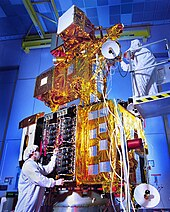
\includegraphics[height=0.1\textheight]{figs/Landsat7photo.jpg}
        \caption{Landsat}
    \end{subfigure}
    \caption{Several Satellites}
\end{figure}
Currently, remote sensing technology is widely used in various fields such as environmental monitoring\cite{li2020review}, urban planning\cite{wellmann2020remote}, resource management\cite{kumar2015applications}, and disaster warning\cite{gupta2022smart}. With continuous technological advancements, the spatial resolution, spectral resolution, and temporal resolution of remote sensing data have significantly improved. In particular, the development of hyperspectral remote sensing and Synthetic Aperture Radar (SAR)\cite{Syntheti6:online} technology has further expanded the precision and scope of remote sensing applications.

\subsection{Development and Application of Big Data}

The rapid development of big data technology has had a profound impact on various fields. Big data typically refers to data sets that cannot be processed using traditional database tools and are characterized by their large volume, variety of data types, high velocity of processing, and high value. Big data technology encompasses multiple stages, including data collection, storage, processing, analysis, and visualization, involving distributed computing frameworks like Hadoop and Spark, as well as data analysis methods such as machine learning and data miningc\cite{mandalImpactAgriculturalManagement2022}.

In the agricultural sector, the application of big data technology includes the collection and analysis of agricultural production data, monitoring and prediction of meteorological data, and analysis and forecasting of market information. Through comprehensive analysis of these data, scientific decision support can be provided for agricultural production, improving production efficiency and reducing resource waste and environmental pollution.

\subsection{Definition and Development of Agricultural Remote Sensing}

Agricultural remote sensing refers to the use of remote sensing technology to acquire and analyze various information in agricultural production to support scientific decision-making in agriculture. The development of agricultural remote sensing can be traced back to the 1960s, when aerial photography technology was primarily used to monitor farmland. With the advancement of satellite remote sensing technology, the application scope and accuracy of agricultural remote sensing have greatly improved.

Modern agricultural remote sensing technology utilizes various platforms, including satellites, drones, and ground sensors, to acquire high-resolution remote sensing data\cite{mullaTwentyFiveYears2013}. By analyzing this data, real-time monitoring of crop growth, pest and disease occurrences, soil moisture, and fertility can be achieved. Agricultural remote sensing technology not only improves agricultural production efficiency but also reduces the use of pesticides and fertilizers, thereby decreasing environmental pollution.

\subsection{The Importance of Agricultural Remote Sensing in Modern Agriculture}

Agricultural remote sensing holds significant application value in modern agriculture. Firstly, it enables real-time monitoring and management of large-scale farmland. Traditional agricultural production management methods often rely on manual surveys and experiential judgments, which are inefficient, costly, and not highly accurate. Remote sensing technology allows for the rapid acquisition of high-precision data over vast areas of farmland, enabling refined management of the fields.

Secondly, agricultural remote sensing technology can improve crop yield and quality. By monitoring crop growth conditions in real time, issues can be promptly identified, and appropriate measures can be taken to prevent the impact of pests, diseases, and adverse environmental factors on crops\cite{kasampalisContributionRemoteSensing2018}. Additionally, remote sensing technology can be used for crop yield prediction, providing a scientific basis for agricultural production.

Lastly, agricultural remote sensing technology plays an important role in environmental protection. Through remote sensing technology, the usage of soil and water resources can be monitored, the impact of agricultural production on the environment can be assessed, and scientific resource management and environmental protection strategies can be formulated.